\documentclass[12pt,a4paper]{article}
\usepackage{rmpackages}																% usual packages
\usepackage{rmtemplate}																% graphic charter
\usepackage{rmexocptce}																% for DS with cptce eval

%\cfoot{} 													% if no page number is needed
%\renewcommand\arraystretch{1.5}		% stretch table line height

\begin{document}

\begin{header}
Préparation de TP

Son et musique
\end{header}

L'objectif de ce TP est de caractériser le son produit par plusieurs instruments : la voix, le diapason, la guitare, etc.

\begin{enumerate}
\item \app{}
\label{quest:diapason}

D'après les documents, quelle est la fréquence de la note émise par un diapason ?

\item \app{}

En vous aidant des documents, proposer une formule permettant de calculer la fréquence $f$ d'un signal périodique d'après la valeur de sa période $T$.

\emph{Aide :}
\begin{center}
\begin{tabular}{c|c}
1 période & $T$ \\
\hline
$f$ périodes & \unit{1}{s}
\end{tabular}
\end{center}
\emph{Le chapitre 12 du livre (page 209--211) vous permettra de vérifier votre réponse.}

\item \rea{} \anarai{}

Avec un smartphone et en vous aidant du document~\ref{doc:phyphox}, réalisez l'acquisition de votre voix : 
\begin{itemize}
\item[•] en répétant rapidement \og La physique, c'est fantastique !\fg{} ;
\item[•] alors que vous bloquez sur le \og i \fg{} de physique : \og La physiiiiiiiiiiiiiiiiiiiiiiiiiiiiiiiiiiiiiiiiiii... \fg{}.
\end{itemize}
Lequel de ces sons est associé à un signal périodique ?
Justifier.

\item \rea{}

Reproduire l'allure d'une période sur votre compte-rendu.

\item \rea{}

Mesurer la période $T$ du signal périodique.
Comment réaliser la mesure la plus précise possible ?
\end{enumerate}

\vfill

\begin{center}
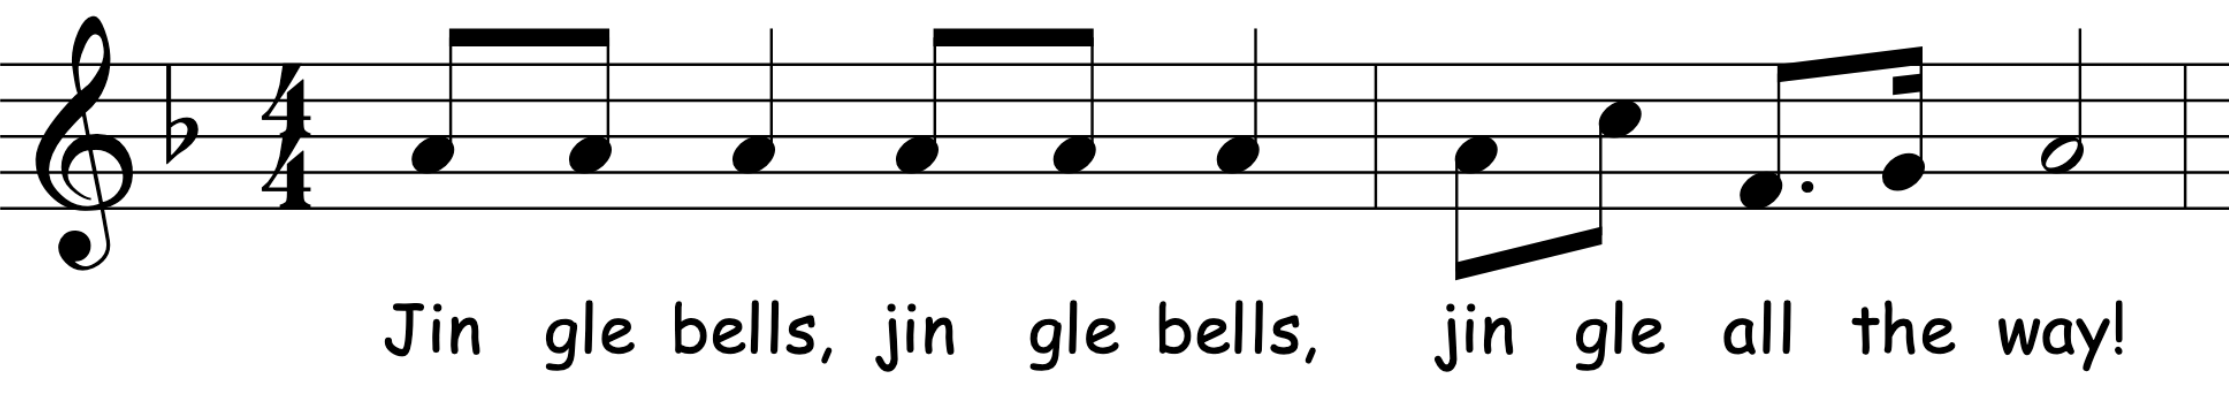
\includegraphics[scale=0.35]{images/jingle_bells.png}
\end{center}

\newpage

%%%%%%%%%%%%%%%%%%%%%%%%%%%%%
% DOCUMENTS
%%%%%%%%%%%%%%%%%%%%%%%%%%%%%

\begin{doc}
\label{doc:phyphox}
\textbf{Acquisition d'un signal sonore avec l'application Phyphox}

Lancer l'application Phyphox (disponible sur Androïd \href{https://play.google.com/store/apps/details?id=de.rwth_aachen.phyphox&hl=fr&gl=US}{https://tinyurl.com/y7fpzd55} et iOS \href{https://apps.apple.com/fr/app/phyphox/id1127319693#?platform=iphone}{https://tinyurl.com/yd56x48k}), orienter le smartphone en mode paysage (à l'horizontale) pour plus de confort d'utilisation puis choisir l'expérience \emph{Mesure du son}.
L'écran du smartphone doit alors être similaire à l'image de gauche ci-dessous.

\begin{center}
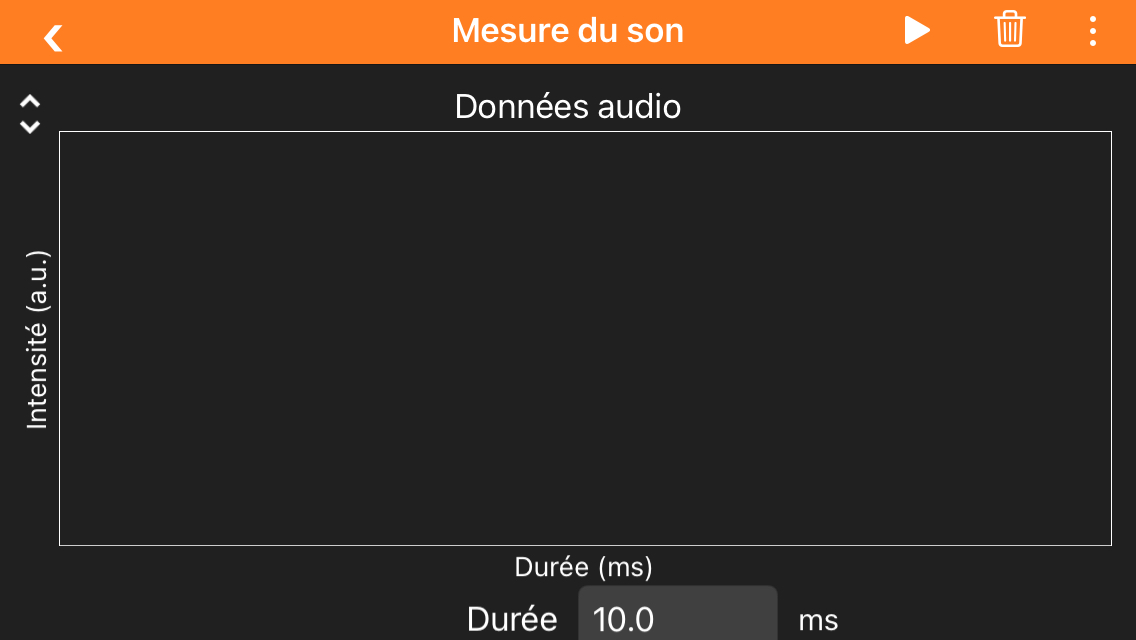
\includegraphics[scale=0.2]{images/phyphox1.jpeg}
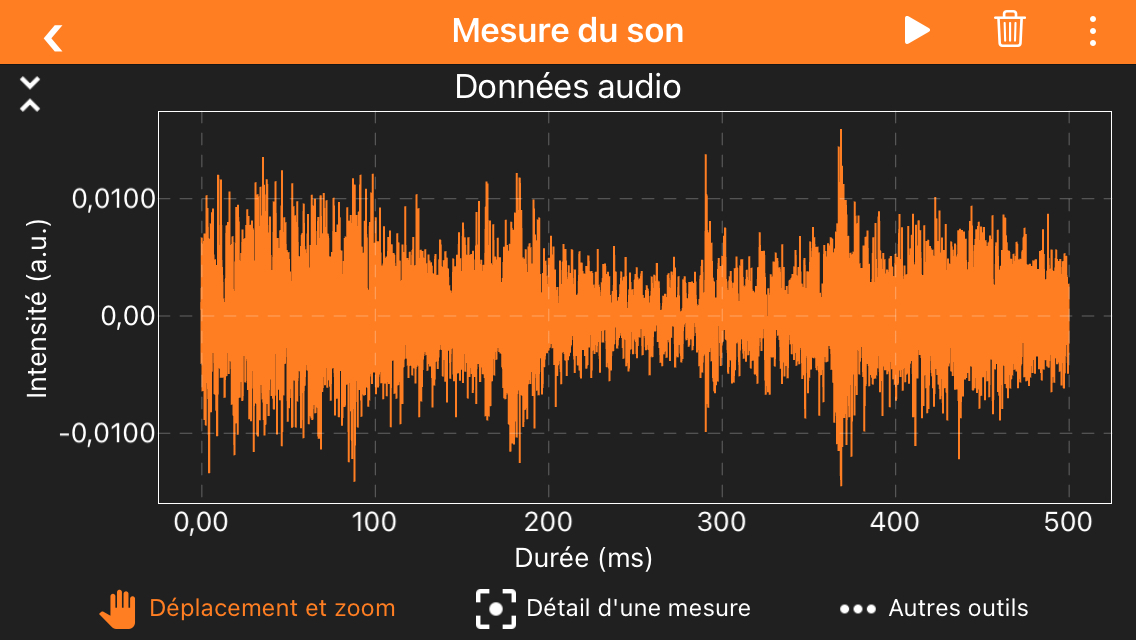
\includegraphics[scale=0.2]{images/phyphox2.jpeg}
\end{center}

\vspace{-2\baselineskip}
\begin{multicols}{2}
\textbf{Réaliser une acquisition}
\begin{enumerate}
\item Modifier la durée d'acquisition : appuyer sur le cadre situé sous le graphe, à côté de \emph{Durée} et rentrer la valeur voulue.
Choisir \unit{200}{ms} pour démarrer.
\item Appuyer sur le bouton 
\includegraphics[height=0.75\baselineskip]{images/phyphox_play.jpeg} pour démarrer l'acquisition.
\item Appuyer sur le bouton 
\includegraphics[height=0.75\baselineskip]{images/phyphox_pause.jpeg} pour arrêter l'acquisition.
\end{enumerate}
\newpage

\textbf{Faire une mesure}
\begin{enumerate}
\item Appuyer sur le graphe pour accéder à tous les menus.
L'écran du smartphone doit alors être similaire à l'image de droite ci-dessus.
\item Appuyer sur \emph{Déplacement et zoom} pour zoomer sur une partie de l'acquisition.
\item En appuyant sur \emph{Détail d'une mesure}, on peut mesurer des intervalles en faisant un \og toucher glisser \fg{}. 
\end{enumerate}
\end{multicols}
\end{doc}

\begin{doc}
\label{doc:periodic_signal}
\textbf{Signal sonore périodique}

Un signal périodique est un signal qui se reproduit à l'identique à intervalles de temps égaux :
\begin{itemize}
\item[•] la \textbf{période} $T$ correspond à la plus petite durée au bout de laquelle le signal se reproduit.
Elle s'exprime en seconde (s).
\item[•] la \textbf{fréquence} $f$ correspond au nombre de périodes du signal par seconde.
Elle s'exprime en hertz (Hz).
\end{itemize}

Le graphe ci-dessous représente un signal électrique périodique de période $T=\unit{2}{ms}$ et de fréquence $f=\unit{500}{Hz}$.

\begin{center}
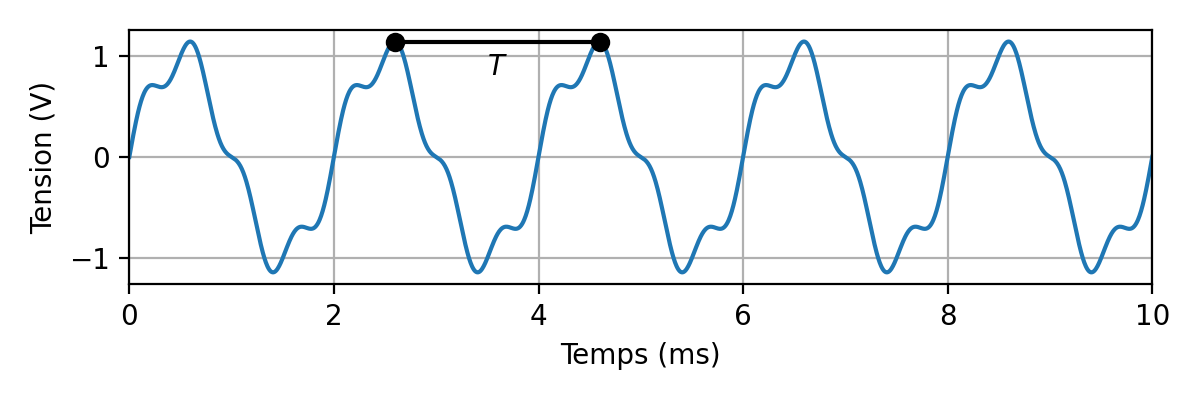
\includegraphics[scale=1]{images/periodic_signal.png}
\end{center}
\end{doc}

\begin{doc}
\textbf{La gamme tempérée}

La musique occidentale est composée avec les notes de la gamme dite tempérée : do, ré, mi, fa, sol, la, si, do à nouveau et ainsi de suite.
Le tableau ci-dessous donne la \textbf{fréquence} de certaines de ces notes :
\begin{center}
\begin{tabular}{l|c|c|c|c|c|c|c|c|c}
\textbf{Note}						& \textbf{Do\textsubscript{1}} & \textbf{Mi\textsubscript{1}} & \textbf{La\textsubscript{1}} & \textbf{Ré\textsubscript{2}} & \textbf{Fa\textsubscript{2}} & \textbf{Sol\textsubscript{2}} & \textbf{Si\textsubscript{2}} & \textbf{Mi\textsubscript{3}} & \textbf{La\textsubscript{3}} \\
\hline
\textbf{Fréquence (Hz)} 	& 65{,}4 & 82{,}4 & 110 & 147 & 175 & 196 & 247 & 330 & 440 \\
\end{tabular}
\end{center}
L'indice situé après le nom de chaque note correspond à l'octave : il permet de différencier le mi grave (Mi\textsubscript{1}) du mi aigu d'une guitare (Mi\textsubscript{3}) par exemple.
\end{doc}

\begin{multicols}{2}
\begin{doc}
\label{doc:diapason}
\textbf{Le diapason}

Le diapason est instrument utilisé pour accorder d'autres instruments.
Une fois frappé, il émet une note unique : le La\textsubscript{3}.
\begin{center}
%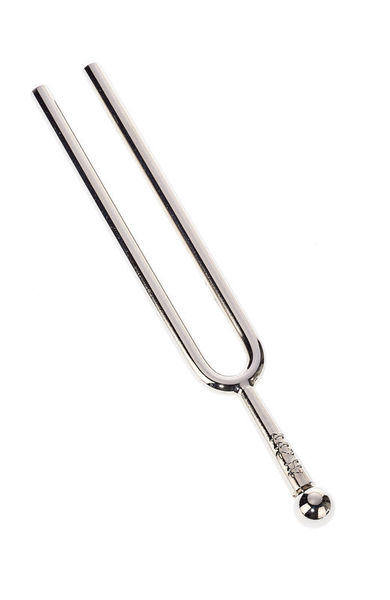
\includegraphics[scale=1.07]{images/diapason.jpg}
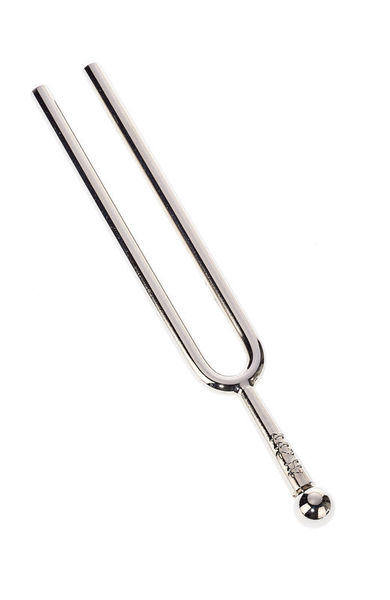
\includegraphics[scale=1.07]{images/diapason.png}
\end{center}
\end{doc}

\begin{doc}
\textbf{La guitare}

Une guitare acoustique possède en général six cordes.
De la corde la plus grave à la plus aigüe, l'accordage standard est :

\begin{center}
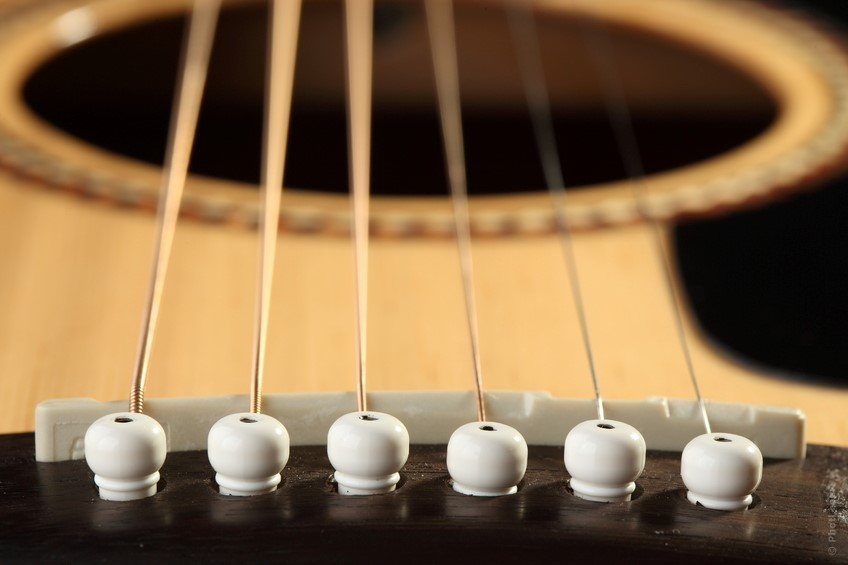
\includegraphics[scale=1]{images/cordes_guitare.jpg}

Mi\textsubscript{1}, La\textsubscript{1}, Ré\textsubscript{2}, Sol\textsubscript{2}, Si\textsubscript{2}, Mi\textsubscript{3}.
\end{center}
\end{doc}
\end{multicols}

\section*{Aide à la rédaction du compte-rendu}

\begin{enumerate}
\item \textbf{Reformuler le problème} en utilisant le vocabulaire scientifique. \hfill \app{}

\item \textbf{Hypothèse}. Donnez votre hypothèse et justifiez-la : \og Je pense que ... car ... \fg{}. \hfill \anarai{}

\item \textbf{Protocole}. \hfill \app{} \anarai{} \rea{}

Mettre en place un protocole pour vérifier votre hypothèse. Il peut contenir :
\vspace{-0.5\baselineskip}
\begin{multicols}{2}
\begin{itemize}
\item[•] une expérience :
\begin{enumerate}
\item liste du matériel ;
\item schémas ;
\item observations et mesures ;
\end{enumerate}
\item[•] un calcul :
\begin{enumerate}
\item formule littérale ;
\item conversion ;
\item application numérique ;
\end{enumerate}
\end{itemize}
\end{multicols}
\vspace{-1.\baselineskip}
\begin{itemize}
\item[•] un raisonnement, une étude de documents, etc.
\end{itemize}
\item \textbf{Conclusion}. Pour terminer le compte-rendu : \hfill \val{}
\begin{itemize}
\item[•] donner les conclusions en reprenant ce qui a été trouvé dans le protocole ;
\item[•] dire si les conclusions sont en accord avec votre hypothèse ;
\item[•] répondre à la question posée !
\end{itemize}
\end{enumerate}

\end{document}

\begin{tabular}{l|c|c|c|c|c|c|c}
\textbf{Note}						& \textbf{Do\textsubscript{1}} & \textbf{Ré\textsubscript{1}} & \textbf{Mi\textsubscript{1}} & \textbf{Fa\textsubscript{1}} & \textbf{Sol\textsubscript{1}} & \textbf{La\textsubscript{1}} & \textbf{Si\textsubscript{1}} \\
\hline
\textbf{Fréquence (Hz)} 	& 65{,}4 & 73{,}4 & 82{,}4 & 87{,}3 & 98{,}0 & 110 & 123 \\
\hline \hline
\textbf{Note}						& \textbf{Do\textsubscript{2}} & \textbf{Ré\textsubscript{2}} & \textbf{Mi\textsubscript{2}} & \textbf{Fa\textsubscript{2}} & \textbf{Sol\textsubscript{2}} & \textbf{La\textsubscript{2}} & \textbf{Si\textsubscript{2}} \\
\hline
\textbf{Fréquence (Hz)} 	& 131 & 147 & 165 & 175 & 196 & 220 & 247 \\
\hline \hline
\textbf{Note}						& \textbf{Do\textsubscript{3}} & \textbf{Ré\textsubscript{3}} & \textbf{Mi\textsubscript{3}} & \textbf{Fa\textsubscript{3}} & \textbf{Sol\textsubscript{3}} & \textbf{La\textsubscript{3}} & \textbf{Si\textsubscript{3}} \\
\hline
\textbf{Fréquence (Hz)} 	& 262 & 294 & 330 & 350 & 392 & 440 & 494
\end{tabular}